% Template created by Karol Kozioł (www.karol-koziol.net) for ShareLaTeX

\documentclass[a4paper,9pt]{extarticle}
\usepackage[utf8]{inputenc}
\usepackage[T1]{fontenc}
\usepackage{graphicx}
\usepackage{xcolor}
\usepackage{tikz}

\usepackage{amsmath,amssymb,textcomp}
\everymath{\displaystyle}

\usepackage{times}
\renewcommand\familydefault{\sfdefault}
\usepackage{tgheros}
\usepackage[defaultmono,scale=0.85]{droidmono}

\usepackage{multicol}
\setlength{\columnseprule}{0pt}
\setlength{\columnsep}{20.0pt}


\usepackage{geometry}
\geometry{
a4paper,
total={210mm,297mm},
left=10mm,right=10mm,top=10mm,bottom=15mm}

\linespread{1.3}


% custom title
\makeatletter
\renewcommand*{\maketitle}{%
\noindent
\begin{minipage}{0.4\textwidth}

\begin{tikzpicture}
\node[rectangle,rounded corners=6pt,inner sep=10pt,fill=blue!50!black,text width= 0.95\textwidth] {\color{white}\Huge \@title};
\end{tikzpicture}
\end{minipage}
\hfill
\begin{minipage}{0.55\textwidth}
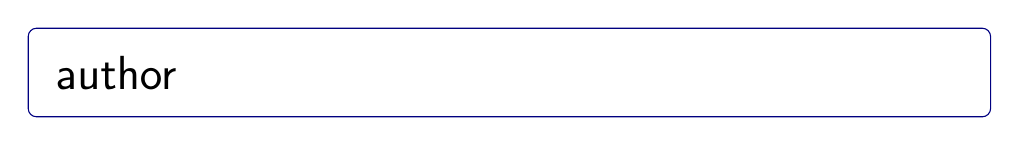
\begin{tikzpicture}
\node[rectangle,rounded corners=3pt,inner sep=10pt,draw=blue!50!black,text width= 0.95\textwidth] {\LARGE \@author};
\end{tikzpicture}
\end{minipage}
\bigskip\bigskip
}%
\makeatother

% custom section
\usepackage[explicit]{titlesec}
\newcommand*\sectionlabel{}
\titleformat{\section}
  {\gdef\sectionlabel{}
   \normalfont\sffamily\Large\bfseries\scshape}
  {\gdef\sectionlabel{\thesection\ }}{0pt}
  {
\noindent
\begin{tikzpicture}
\node[rectangle,rounded corners=3pt,inner sep=4pt,fill=blue!50!black,text width= 0.95\columnwidth] {\color{white}\sectionlabel#1};
\end{tikzpicture}
  }
\titlespacing*{\section}{0pt}{15pt}{10pt}


% custom footer
\usepackage{fancyhdr}
\makeatletter
\pagestyle{fancy}
\fancyhead{}
\fancyfoot[C]{\footnotesize \textcopyright\ \@date\ \ \@author}
\renewcommand{\headrulewidth}{0pt}
\renewcommand{\footrulewidth}{0pt}
\makeatother


\title{Wordnet and FNE}
\author{Raquel Leandra Pérez}
\date{2014}



\begin{document}

\maketitle

\begin{multicols*}{2}


\section{Intro}
\begin{itemize}
\item {\color{blue} Portada }: Hola, soy Raquel y presentaré el trabajo Wordnet y Deep Learning: Una posible 
Unión. Mis directores son Dario Garcia Gasulla y Ulises García.
\item {\color{blue} Estructura }: La estructura del trabajo es muy similar a la de la memoria escrita: 

\begin{itemize}
\item Primero hablaré de los conocimientos necesarios para entender el trabajo, con menos detalle que en la memoria a causa de las limitaciones del tiempo. 
\item Después explicaré el trabajo relacionado con el análisis posterior. 
\item Seguidamente explicaré el enfoque y el análisis.
\item Finalmente comentaré las conclusiones obtenidas.
\end{itemize}

\end{itemize}

\section{Redes Neuronales}
\begin{itemize}
\item {\color{blue} Que explicaré}: En este apartado explicaré a grandes rasgos como funcionan redes neuronales, redes convolucionales 
y transfer learning. 
\item {\color{blue} Una Neurona}: Una red neuronal es un modelo computacional de aprendizaje inspirado en la forma de procesar la 
información del cerebro. 

Su unidad básica de computación es una neurona. Cada neurona actua como una función sobre unas ciertas entradas y genera una salida. En la figura 
podemos ver un ejemplo de neurona. A la izquierda tenemos su entrada, luego los pesos, que se combinan linealmente con la entrada y se transforman utilizando una función de activación no lineal. 

\item {\color{blue} Por capas}: Las neuronas se suelen organizar en capas, las más comunes son las capas \textit{fully-connected}, como la que se ve en la figura. 
En ella podemos ver la estructura base de una red neuronal, donde a la izquierda vemos la entrada, en el centro las capas ocultas, acompañadas de sus correspondientes sesgos y finalmente a la derecha la salida. Por cada arista hay un peso, que se entrena calculando las derivadas parciales utilizando backpropagation y luego minimizando un error utilizando el algoritmo de \textit{Stochastic Gradient Descend}. 

\end{itemize}

\section{Redes Convolucionales}
Las redes convolucionales son muy similares a las redes neuronales explicadas, las mayores diferencias son 
que asumen una estructura concreta en la entrada, y contienen neuronas neuronas convolucionales, es decir, aquellas que operan con 
una convolución, que generalmente opera una función de kernel sobre la imagen, como podemos 
ver en el ejemplo de la figura.  Donde podemos ver a la izquierda la imagen general, en el centro el kernel y a la derecha la convolución resultante. 

En redes convolucionales, la disposición por capas permite representar la información más compleja a
partir de otra más simples. Por tanto puede acabar extrayendo features abstractas, como las que vemos en la segunda figura. 

\section{Transfer Learning}

Otro concepto importante en este trabajo es el de \textit{transfer learning}, que es el campo
de estudio que reutiliza el lenguaje de representación en otro. Puesto a que las redes convolucionales 
tienen una gran cantidad de parámetros, muchas veces es demasiado costoso a nivel de recursos computacionales
o de cantidad de datos para entrenar. Utilizando transfer learning se pueden solventar estos problemas. 
Comúnmente se suele utilizar para:
\begin{itemize}
\item \textbf{fine tuning}, que consiste en tomar los pesos ya entrenados por el conjunto de datos de origen, y a continuación, entrenar la red sobre esta inicialización utilizando el conjunto de datos de la tarea de destino. 
\item O para \textbf{Feature Extraction}, que consiste en procesar un conjunto de datos a través de una red neuronal
ya entrenada y extraer valores de activación para que puedan ser utilizados por otro mecanismo de
aprendizaje. Un ejemplo de estructura básica para feature extraction sería el de la figura.
\end{itemize}

\section{FNE}

En transfer learning para feature extraction generalmente se fijan todas las capas menos las dos últimas, que se entrenan con el nuevo 
conjunto de datos. Sin embargo en este trabajo nos centramos en el Full-network embedding, un embedding que, a diferencia del anterior, 
permite entrenar todas las capas. Creando de esta forma un lenguaje de representación mejor. 
Éste se obtiene con el siguiente algoritmo: 

\begin{itemize}
\item Primero se realiza un fordward pass del conjunto de datos target por toda la red y se guardan los valores de activación de las neuronas. 
\item Seguidamente se le aplica un pooling espacial a estos datos.
\item A continuación se aplica una estandarización a las features.
\item y Finalmente al resultado se le aplica una discretización. 
\end{itemize}

La estructura del proceso sería la que podemos ver en la figura. Donde se extraen las features de todas las capas y se someten al algoritmo para obtener el
embedding final. Que se podría utilizar para la tarea objetivo utilizando algún método, como por ejemplo una SVM. 
\section{Wordnet}

Wordnet es una base de datos que contiene nombres, verbos, adjetivos y adverbios en conjuntos de
sinónimos (que llamaremos synsets).Los synsets están conectados entre ellos por medio de relaciones
conceptuales, semánticas y léxicas. Como serían la de sinonimia, hiponimia e hiperonimia.
 
\section{Imagenet}
Imagenet es una base de datos de imágenes organizada utilizando la jerarquía de wordnet. Su principal
objetivo es dotar a los investigadores en campos relacionados con visión artificial de una base de datos a gran
escala con la que poder trabajar.

Para el full-network embedding utilizaron el subconjunto correspondiente al reto de imagenet de 2012
de reconocimiento de imágenes.
Éste consta de:
\begin{itemize}
\item Un conjunto de datos de entrenamiento de 1.2 millones de muestras y 1,000 categorías diferentes.
\item Un conjunto de datos de validación de 50,000 muestras y 1,000 categorías.
\end{itemize}

\section{Datos iniciales}
En nuestro caso estudiaremos un full-network embedding obtenido a partir de la tarea origen (T S =Clasificación
de imágenes, D S = 1.2 M imágenes de Imagenet con sus correspondientes clases) y una tarea de destino
(T T =Clasificación de imágenes, D T = 50,000 imágenes de Imagenet con sus correspondientes clases).

Es decir, partiendo de una red convolucional entrenada con todo el conjunto de datos de entrenamiento
de Imagenet, hemos generado un lenguaje de representación para el conjunto de datos de validación de
Imagenet. Lo que resulta en el full-network embedding con el que trabajaremos.
El full-network embedding consiste en una matriz de tamaño 50,000 muestras por 12,416 características,
como observamos en la figura.


\section{Objetivos}
Los objetivos del análisis que haremos son: 
\begin{itemize}
\item Analizar el \textit{embedding} dado y el comportamiento de las \textit{features} en las distintas capas.
\item Analizar si hay alguna relación entre el \textit{embedding} y los \textit{synsets} seleccionados.
\end{itemize}
Respecto a los \textit{synsets} que analizaremos, hemos elegido los siguientes por estar distribuidos de una forma bastante uniforme entre las
clases, y por ser de dos ''ramas'' lo más diferentes posibles,además representan niveles de abstracción parecidos.

\section{Estadísticas}

\section{Hipótesis}

\section{De WN a FNE}

\section{synsets}

\section{De FNE a WN}

\section{Conclusiones }

\end{multicols*}

\end{document}
